\subsection{\arp}


\subsubsection{Wstęp}

\arp{} -- \emph{Address Resolution Protocol} jest protokołem umożliwiającym
współpracę pomiędzy drugą a trzecią warstwą modelu OSI. Jest wykorzystywany do
znajdywania adresów maszyn w warstwie łącza, na podstawie ich adresów w warstwie
sieci. W wykonanym ćwiczeniu znajdowany zostaje adres MAC maszyny, posiadając
jej adres IPv4.

Zasada działania protokołu \arp{} jest stosunkowo prosta. W systemach
operacyjnych protokół obsługiwany jest przeważnie przez program \texttt{arp}.
Gdy adres fizyczny maszyny\dywiz adresata jest nieznany, wysyłane jest zapytanie
\arp. Jest to ramka \eth{} zawierająca adres IP adresata. Ramka jest prośbą o
odpowiedź od maszyny, która ma przypisany dany adres IP
\cite{arp:stevens-przyklad}. Zapytanie jest wysyłanie jako \emph{broadcast}
na warstwie łącza aktualnej podsieci.

Dla polepszenia wydajności zarządzania połączeniami, program \texttt{arp}
przechowuje w pamięci podręcznej tablicę mapującą adresy logicznie na adresy
fizyczne. Wpis jest uznawany za poprawny przez okres 20 minut, następnie zostaje
odświeżony \cite{arp:stevens-cache}.

W sieciach IPv6 funkcjonalność \arp{} spełnia protokół NDP -- \emph{Neighbor
Discovery Protocol}. W połączeniach \ppp{} i innych połączeniach point-to-point
protokół \arp{} nie jest potrzebny.


\subsubsection{Wykonanie ćwiczenia}

Korzystano z maszyn \tjz{} (\texttt{t10}) oraz \tjj{} (\texttt{t11}) połączonych
bezpośrednio kablem \eth. Schemat nr~\ref{fig:arp:schemat_po_konfiguracji}
przedstawia wykorzystane połączenia.

\begin{figure}[h!]
  \centering
  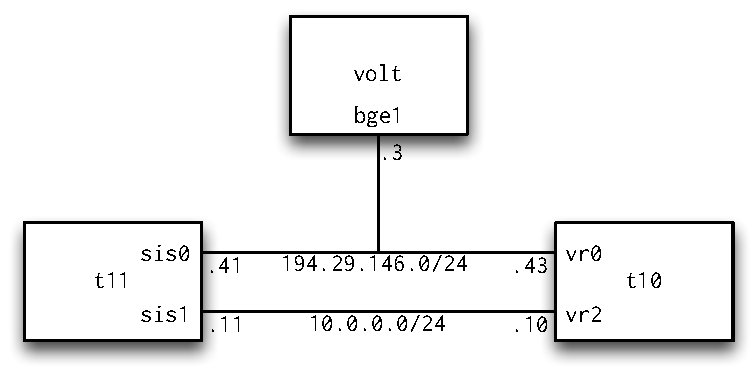
\includegraphics[width=11cm]{figury/arp/schemat-po-konfiguracji.pdf}
  \caption{Schemat sieci IPv4 do obserwacji \arp.}
  \label{fig:arp:schemat_po_konfiguracji}
\end{figure}

Interfejsy maszyn należące do sieci \texttt{194.29.146.0/24} tj. \texttt{sis0}
oraz \texttt{vr0} odpowiednio dla maszyn \tjz{} oraz \tjj, zostały
prekonfigurowane podczas podnoszenia systemu operacyjnego. Sieć
\texttt{10.0.0.0/24} została skonfigurowana do obserwacji pakietów protokołu
\arp. Na obu maszynach ręcznie skonfigurowano interfejsy, oraz upewniono się, że
pamięć podręczna \texttt{arp} jest pusta.

Można zauważyć, że w przeciwieństwie do wpisów dla adresów innych maszyn, adresy
przypisane do interfejsów bieżącej maszyny są zapamiętywane bez limitu
czasowego.

\begin{lstlisting}
so5501b% sudo ifconfig vr2 10.0.0.10/24
so5501b% sudo arp -d -i vr2 -a
so5501b% arp -i vr2 -a
? (10.0.0.10) at SO5501B2 on vr2 permanent [ethernet]
\end{lstlisting}

\begin{lstlisting}
so4801% sudo ifconfig sis1 10.0.0.11/24
so4801% sudo arp -d -i sis1 -a
so4801% arp -i sis1 -a
? (10.0.0.11) at SO4801B on sis1 permanent [ethernet]
\end{lstlisting}

Włączono nasłuchiwanie pakietów \arp{} na \tjj{} i przesłano jedno zapytanie
\texttt{ping} z maszyny \tjz.

\begin{lstlisting}
so5501% ping -c 1 10.0.0.11
\end{lstlisting}

\begin{lstlisting}
so4801% sudo tcpdump -i sis1 arp
listening on sis1, link-type EN10MB (Ethernet), capture size 65535 bytes
17:08:50.072670 ARP, Request who-has 10.0.0.10 tell 10.0.0.11, length 28
17:08:50.072865 ARP, Reply 10.0.0.10 is-at SO5501B2, length 46
17:13:16.147967 ARP, Request who-has 10.0.0.11 tell 10.0.0.10, length 46
17:13:16.148178 ARP, Reply 10.0.0.11 is-at SO4801B, length 28
\end{lstlisting}

W listingu widoczne są dwie wymiany \texttt{Request/Reply}. Pierwsza pochodzi z
maszyny \tjz{} szukającej maszyny \tjj{}, by wysłać zapytanie z \texttt{ping}.
Druga wymiana jest z maszyny \tjj{}, by móc odpowiedzieć na \texttt{ping}. Efekt
wymian jest widoczny w tablicy pamięci podręcznej \texttt{arp}, jako ostatni
wpis o ograniczonym czasie życia.

\begin{lstlisting}
so4801% arp -i sis1 -a
? (10.0.0.11) at SO4801B on sis1 permanent [ethernet]
? (10.0.0.10) at SO5501B2 on sis1 expires in 1147 seconds [ethernet]
\end{lstlisting}
